\let\negmedspace\undefined
\let\negthickspace\undefined
\documentclass[journal]{IEEEtran}
\usepackage[a5paper, margin=10mm, onecolumn]{geometry}
\usepackage{lmodern} % Ensure lmodern is loaded for pdflatex
\usepackage{tfrupee} % Include tfrupee package

\setlength{\headheight}{1cm} % Set the height of the header box
\setlength{\headsep}{0mm}     % Set the distance between the header box and the top of the text

\usepackage{gvv-book}
\usepackage{gvv}
\usepackage{cite}
\usepackage{amsmath,amssymb,amsfonts,amsthm}
\usepackage{algorithmic}
\usepackage{graphicx}
\usepackage{textcomp}
\usepackage{xcolor}
\usepackage{txfonts}
\usepackage{listings}
\usepackage{enumitem}
\usepackage{mathtools}
\usepackage{gensymb}
\usepackage{comment}
\usepackage[breaklinks=true]{hyperref}
\usepackage{tkz-euclide} 
\usepackage{listings}
\usepackage{gvv}                                        
\def\inputGnumericTable{}                                 
\usepackage[latin1]{inputenc}                                
\usepackage{color}                                            
\usepackage{array}                                            
\usepackage{longtable}                                       
\usepackage{calc}                                             
\usepackage{multirow}                                         
\usepackage{hhline}                                           
\usepackage{ifthen}                                           
\usepackage{lscape}
\begin{document}

\bibliographystyle{IEEEtran}
\vspace{3cm}

\title{12.9.ex.1.1}
\author{EE24BTECH11003 - Akshara Sarma Chennubhatla}
% \maketitle
% \newpage
% \bigskip
{\let\newpage\relax\maketitle}
\textbf{Question:}
Solve the differential equation $\frac{dy}{dx} - \cos x = 0$, with the initial condition $y\brak{0} = 0$\\

\solution\\
\textbf{Theoretical Solution:}\\

\begin{align}
	\frac{dy}{dx} &= \cos x\\
\end{align}
Integrating on both sides,
\begin{align}
	\int{\frac{dy}{dx}} dx &= \int{\cos x} dx\\
	y &= \sin x + C\\
\end{align}
Since $\brak{0, 0}$ satisfies the function,
\begin{align}
	0 &= \sin\brak{0} + C\\
	\implies 0 &= 0 + C\\
	\implies C &= 0\\
\end{align}
So the function $y\brak{x}$ is,
\begin{align}
	y &= \sin x\\
\end{align}

\textbf{Simulated Solution:}\\
The method being used here is the Bilinear Transform\\
First step is to apply Laplace Transform on both sides of the equation\\
Laplace transform by definition is,
\begin{align}
	\mathcal{L}\brak{f\brak{t}} = \int_0^{\infty} e^{-st} f\brak{t} dt
\end{align}
Properties of Laplace Transform used here are,
\begin{align}
	\mathcal{L}\brak{\cos{t}} &= \frac{s}{s^2 + 1}\\
	\mathcal{L}\brak{y^\prime} &= s\mathcal{L}\brak{y} - y\brak{0}\\
\end{align}
By applying Laplace Transform,
\begin{align}
	\mathcal{L}\brak{\frac{dy}{dx}} &= \mathcal{L}\brak{\cos x}\\
	sY\brak{s} - y\brak{0} &= \frac{s}{s^2 + 1}\\
\end{align}
By taking $y\brak{0} = 0$,
\begin{align}
	Y\brak{s} = \frac{1}{s^2 + 1}
\end{align}
Applying Bilinear transform, with $T = h$, we get,
\begin{align}
	s &= \frac{2}{T}\frac{1 - z^{-1}}{1 + z^{-1}}\\
	&= \frac{2}{h}\frac{1 - z^{-1}}{1 + z^{-1}}\\
	Y\brak{z} &= \frac{1}{\brak{\frac{2\brak{1 - z^{-1}}}{h \brak{1 + z^{-1}}}}^2 + 1}\\
	Y\brak{z} &= \frac{h^2\brak{z + 1}^2}{4\brak{z - 1}^2 + h^2\brak{z + 1}^2}\\
	Y\brak{z}\brak{\brak{4 + h^2}\brak{z^2 + 1} + \brak{h^2 - 4}2z} &= h^2\brak{z^2 + 1 + 2z}\\
	z^2 Y\brak{z}\brak{4 + h^2} + Y\brak{z}\brak{4 + h^2} + 2z Y\brak{z}\brak{h^2 - 4} &= h^2\brak{z^2 + 1 + 2z}\\
\end{align}
Properties of one sided $z$ transform used here are,
\begin{align}
	\mathcal{Z}\brak{y\sbrak{n + 2}} &= z^2 Y\brak{z} - y\sbrak{1}z - y\sbrak{0}\\
    	\mathcal{Z}\brak{y\sbrak{n + 1}} &= z Y\brak{z} - z y_\sbrak{0}\\
    	\mathcal{Z}\brak{y\sbrak{n}} = Y\brak{z} &\implies \mathcal{Z}\brak{y\sbrak{n - n_0}} = z^{-n_0}Y\brak{z} \label{time_shift_eq}
\end{align}
By the time shift property $\brak{\ref{time_shift_eq}}$,
\begin{align}
	\mathcal{Z}\brak{\delta\sbrak{n + 2}} &= z^2 \text{, } z \neq 0\\
	\mathcal{Z}\brak{\delta\sbrak{n + 1}} &= z \text{, } z \neq 0\\
	\mathcal{Z}\brak{\delta\sbrak{n}} &= 1\\
\end{align}
By rewriting the equation,
\begin{align}
	z^2 \brak{Y\brak{z} - y\brak{1}z - y\brak{0}}\brak{4 + h^2} + Y\brak{z}\brak{4 + h^2} + \\2\brak{z Y\brak{z} - zy\brak{0}}\brak{h^2 - 4}  + \brak{4 + h^2}\brak{y\brak{1}z + y\brak{0}} + 2zy\brak{0}\brak{h^2 - 4} &= h^2\brak{z^2 + 1 + 2z}\\
\end{align}
For plotting the above difference equation, we need $y_0 = y\brak{0}$ as well as $y_1$. To find $y_1 = y\brak{0 + h} = y\brak{h}$ we employ first principle of derivative,
\begin{align}
    	y^{\prime}\brak{x} &= \lim_{h\to0} \frac{y\brak{x + h} - y\brak{x}}{h}\\
    	y\brak{x + h} &= y\brak{x} + hy^{\prime}\brak{x}, h\to0\\
    	y_1 &= y\brak{h} = y\brak{0} + hy^{\prime}\brak{0}\\
	y_1 &= 0 + h \cos\brak{0}\\
	y_1 &= h
\end{align}
Taking $z$ inverse transform on both sides of the equation, we get the difference equation which is,
\begin{align}
	\brak{y_{n+2} + y_n}\brak{4 + h^2} + 2\brak{h^2 - 4}y_{n+1} + h\brak{4 + h^2}\delta\brak{n} = h^2\brak{\delta\brak{n+2} + \delta\brak{n} + 2\delta\brak{n+1}}
\end{align}
Here, $\delta$ is given by,
\begin{align}
	\delta\brak{n - n_0} =
	\begin{cases}
		1 & \quad n = n_0\\
        	0 & \quad n \neq n_0
    	\end{cases}
\end{align}
As $n > 0$, 
\begin{align}
    	\delta\brak{n + 2} = \delta\brak{n + 1} = 0
\end{align}



Below is the simulated plot and the theoretical plot for given curve based on initial conditions, $x_0 = 0, y_0 = 0, y_1 = h$, obtained by iterating through the values of $x$ with step size of $h$
\begin{figure}[h!]
	\centering
	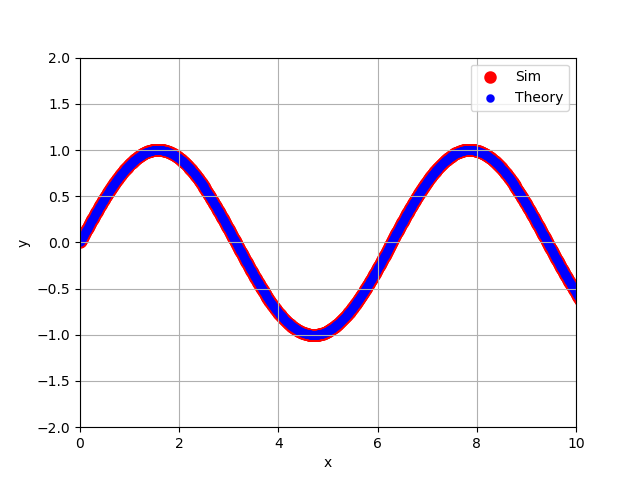
\includegraphics[width=1\columnwidth]{figs/simulated.png}
	\caption{Plot of the solution of $\frac{dy}{dx} - \cos x = 0$}
	\label{stemplot}
\end{figure}

\end{document}
